\documentclass[amssymb,twocolumn,aps]{revtex4}

% allows special characters (including æøå)
\usepackage[utf8]{inputenc}
%\usepackage [norsk]{babel} %if you write norwegian
\usepackage[english]{babel}  %if you write english

\usepackage{physics,amssymb}  % mathematical symbols (physics imports amsmath)
\usepackage{graphicx}         % include graphics such as plots
\usepackage[table]{xcolor}
\usepackage{xcolor}           % set colors
\usepackage{hyperref}         % automagic cross-referencing 
\usepackage{float}			  % force placement of tables and figures
\usepackage{comment}
%\usepackage[authoryear]{natbib}


\begin{document}

\title{Report Template \\
    \normalsize FYS-STK3155 - Project X}
\date{\today}               
\author{
    Anton Nicolay Torgersen 
}
\affiliation{University of Oslo}


\newpage


%Abstract: accurate and informative? Total number of possible points: 5

    \begin{abstract}
A study of various regression methods, including OLS, Ridge and LASSO and how they fit Runge's function. 
We review the theory and implementation of these methods and see how they compare on this function.
At the end, we discuss some resampling techniques on the simpler OLS-method to understand the bias-variance trade-off.
\end{abstract}


    \maketitle
    \thispagestyle{empty} % Removes page number from the title page

    


% Introduction: status of problem and the major objectives. Total number of possible points: 10
\section{Introduction}

The fundamental problem in machine learning and statistics is to find meaningful patterns in data using models that make accurate predictions on unseen data.
This is a difficult task, as a complex function might fit the training data perfectly, but fail spectacularly when facing new instances, a phenomenon known as overfitting.
On the other hand a model that is too simple may fail to extract the patterns in the data and thus underfit the data.
Therefore understanding of the bias-variance tradeoff on simpler models before the more complex ones is paramount to develop robust and generalizable models.

Therefore, this paper will study the bias-variance tradeoff through the lens of regression models, that increase in complexity.
We start with the simplest model, Ordinary Least Squares (OLS), where we have a fully analytical solution for the best fit parameters.
Then we move on to Ridge regression, which is a regularized version of OLS, where we first introduce the tuning of a penalization parameter $\lambda$ to find a good balance between bias and variance.
Finally we end with LASSO regression, which is another regularized version of OLS, but with a different penalization term.

This analysis will closely follow the lecture notes from FYS-STK3155 \cite{compfys} and the book "The Elements of Statistical Learning" by Hastie, Tibshirani and Friedman \cite{hastie}.
We will review the theory of the three regression methods and apply the methods to a one-dimensional problem, fitting a polynomial model to Runge's function, $f(x)=1/(1+25x^2)$.
This function is notoriously difficult for high-degree polynomial interpolation and will therefore be a good demonstration of the pitfalls of overfitting and the benefits of regularized techniques like Ridge and LASSO.
Together these three models will create a better understanding of the dynamics between bias and variance, how the dynamic shifts with model complexity and methods.
The result is a better intuition for tuning models, when is the model inching towards the true function $y$ and when is it stuck in a well. 


\begin{comment}
When you write the introduction you should focus on the following aspects:
\begin{itemize}
    \item Motivate the reader, the first part of the introduction gives always a motivation and tries to give the overarching ideas. Citing some central ideas or problems in the literature is a good idea here. \cite{compfys}\cite{eigenvalue}\cite{hein, hastie}
    \item What you have done, with a focus on choice of problem and method, and why these were chosen.
    \item The structure of the report, how it is organized. List the sections, and very briefly describe what is in them and how they fit together.
\end{itemize}
\end{comment}

\section{Methods}\label{section:methods}
We will be assuming that the reader has some familiarity with linear algebra and multivariable calculus.
For a more in-depth review of the methods and algorithms, including the motivation for using them and their applicability to the problem, please refer to the lecture notes \cite{compfys} and the book "The Elements of Statistical Learning" by Hastie, Tibshirani and Friedman \cite{hastie}.
For the scoring measures Mean Squared Error (MSE) and R2, please refer to \cite{scoring1} section 2.2.1 and 3.1.3 for information or see the implementation in the code.

\subsection{Regression Methods}
We will be studying three regression methods: Ordinary Least Squares (OLS), Ridge regression and LASSO regression.
All three methods are used to fit a polynomial model to the data, but they differ in how they estimate the model parameters and how they handle overfitting.

The problem we are tyring to solve is to find a polynomial function $\tilde{y}(x)$ that approximates the true function $y(x)$, given a set of data points $(x_i, y_i)$, where $i=1,2,...,n$.

\subsubsection{Ordinary Least Squares (OLS)}
The simplest of the three methods, it is defined by minimizing the sum of the squared differences between the observed values $y_i$ and the predicted values $\tilde{y}_i$.

$$\frac{1}{n} \sum_{i=1}^{n} (y_i - \tilde{y}_i)^2$$

where $\tilde{y} = X\theta$, $X$ is the design matrix, $\theta$ is the vector of model parameters and $y$ is the vector of observed values.

Taking the derivative with reagrds to $\theta$ equal to $0$ gives rise to an analytical solution with no relance on $\theta$:
\begin{equation}
  \theta = (X^TX)^{-1}X^Ty  
\end{equation}
This solution is valid as long as $X^TX$ is invertible, which is the case when the columns of $X$ are linearly independent, and if they are not one can just shift the diagonal slightly.

We also have a gradient descent solution to this problem by taking the derivative of the cost function with reagrds to $\theta$ and updating $\theta$ iteratively.
\begin{align}
\nabla_{\theta_n} &= \frac{1}{n}2X^T(X\theta_n + y) \\
\theta_{n+1} &= \theta_n - \eta \nabla_{\theta_n}
\end{align}
where $\eta$ is the learning rate that controls the step size in the parameter space.

\subsubsection{Ridge Regression}
This is a regularized version of OLS, where we add a penalization term to the cost function to prevent overfitting.
\begin{equation}
    \frac{1}{n} \sum_{i=1}^{n} (y_i - \tilde{y}_i)^2 + \lambda \sum_{j=1}^{p} \theta_j^2
\end{equation}

where $\lambda$ is the regularization parameter that controls the strength of the penalization and $p$ is the number of model parameters, in our case the degree of the polynomial.
The analytical solution is given by:
\begin{equation}
\theta = (X^TX + \lambda I)^{-1}X^Ty
\end{equation}
where $I$ is the identity matrix.

We also have a gradient descent solution to this problem by taking the derivative of the cost function with reagrds to $\theta$ and updating $\theta$ iteratively.
\begin{align}
\nabla_{\theta_n} &= \frac{1}{n}2X^T(X\theta_n + y) + 2\lambda \theta_n \\
\theta_{n+1} &= \theta_n - \eta \nabla_{\theta_n}
\end{align}

\subsubsection{LASSO Regression}
part f, algorithm, cost function

For more on these three methods see \cite{compfys} and \cite{hastie}.

\subsection{Gradient Descent}

\subsubsection{Stochastic Gradient Descent}
part f, write about the theory?


\subsection{Sampling methods}
part g, write about the implementation of the bootstrap method as a resampling technique on the OLS method.
part h, write about the implementation of the k-fold cross-validation algorithm as a resampling technique on the OLS, Ridge and LASSO methods.

\begin{comment}
\begin{itemize}
    \item Describe the methods and algorithms, including the motivation for using them and their applicability to the problem
    \item Derive central equations when appropriate, the text is the most important part, not the equations.
\end{itemize}
\end{comment}
\subsection{Implementation}
To evaluate the performance of the regression methods and to elucidate the intricacies of the methods and the bias-variance tradeoff we are using Runge's function as a test case.
This is a one-dimensional function

$$
f(x) = \frac{1}{1 + 25x^2},
$$

that is know to be difficult to fit with high-degree polynomials.

We will generate two a data sets of $n$ points, $x_i$, uniformly distributed in the interval $[-1, 1]$, one with and one without noise.
The noisy data set will be generated by adding Gaussian noise $\epsilon_i \sim \mathcal{N}(0, \sigma^2)$ to the function values.


\begin{figure*}[t]
    \centering
    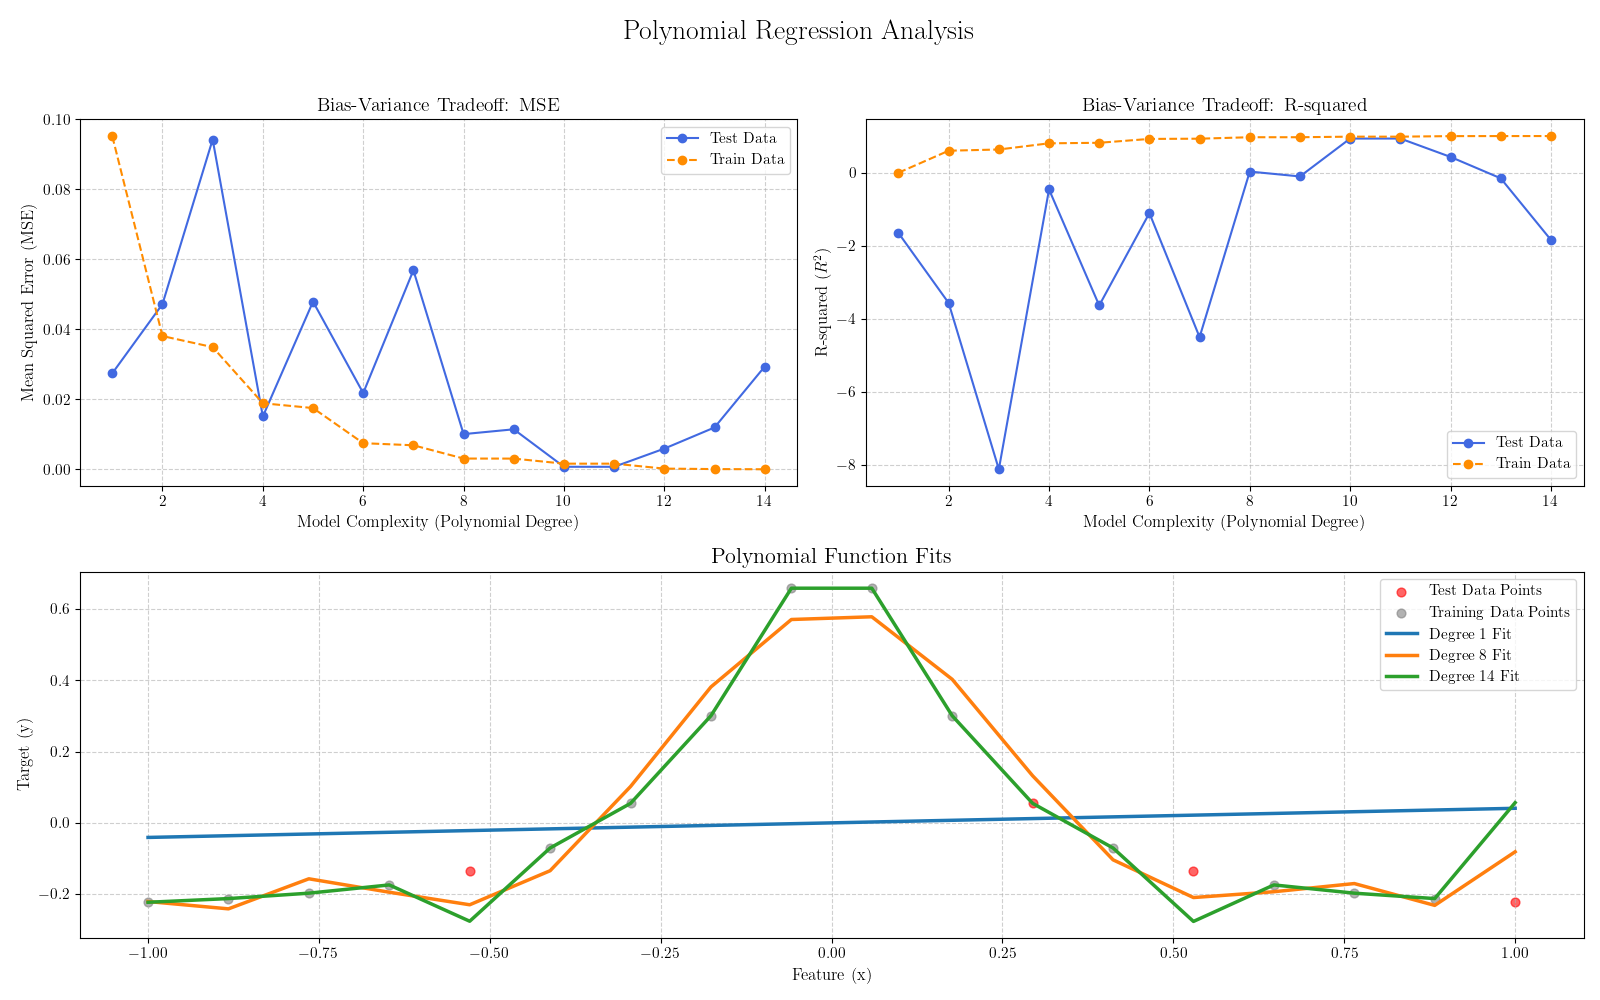
\includegraphics[width=.95 \textwidth]{Figures/Combined_Analysis_OLS.png}
    \caption{OLS and model complexity with 14 training datapoints}
    \label{fig:OLS1}
\end{figure*}
Implementation of the analytical solution of OLS regression using the numpy function pinv {citation???}.
\subsubsection{Regression methods}

perhaps simply a reference to the code for the implementation using numpy.
And a test with the scikit library to see that the implementation is correct for these two.

Maybe some extra for the Lasso implementation?

\subsubsection{Gradient Descent}
part c, write about how we implementation of the gradient descent algorithm for OLS and Ridge regression.
Again squeez it tohether we the above section and reference the code and functions.

\subsubsection*{Changing learning rate}
part,d implementation of the changing learning rate algorithms: momentum, ADAgrad, RMSprop and Adam.
Follows the implementations from the lecture notes from week 37 \cite{compfys} and is explained in the code.
Function  bla bla bla


\subsubsection*{Stochastic Gradient Descent}
part f, write about the implementation of the stochastic gradient descent algorithm for OLS and Ridge regression.

\subsubsection{Resampling techniques}
part g, write about the implementation of the bootstrap method as a resampling technique on the OLS method.

PROBABLY NOT.part h, write about the implementation of the k-fold cross-validation algorithm as a resampling technique on the OLS, Ridge and LASSO methods.


\begin{comment}
\begin{itemize}
    \item Explain how you implemented the methods and also say something about the structure of your algorithm and present very central parts of your code, not more than 10 lines
    \item You should plug in some calculations to demonstrate your code, such as selected runs used to validate and verify your results. A reader needs to understand that your code reproduces selected benchmarks and reproduces previous results, either numerical and/or well-known closed form expressions.
\end{itemize}
\end{comment}


\subsection{Use of AI tools}
	AI has been used to format and proofread the report and to spot errors in the code.
\begin{itemize}
    \item Describe how AI tools like ChatGPT were used in the production of the code and report.
\end{itemize}

\newpage



\section{Results and Discussion}\label{section:results}

Description of the function, why it is interesting to study.



Generation of the data set and why and how we scaled it. ( part a)
We had a set with and without noise in a normal distribution to see how the methods performed on both.


Analysis using the methods described in section \ref{section:methods}.

\subsection{Regression methods}

\subsubsection{Ordinary Least Squares (OLS)}

We first analyzed how OLS works on a small dataset as with more data the variances in training is harder to see. In the figure \ref{fig:OLS1} we see that the data that it trains one becomes better and better the more complex the model becomes as it then has more parameters to model the data on. While the test data becomes much worse when the complexity is close to the number of data points. This implies that the training now fits the points rather than the underlying curve.

\textbf{some thoughts on the R2}


Analyzing how the relationship between datapoints and training at figure\ref{fig:OLSHeat} we see, as we expect, along the borders where there is low training data or low complexity are the worst performing parts on the test data. The yellow spots in the heatmap are capped at 0.1, as these points are prone to explode just as the graph \ref{fig:OLS1} is beginning to do.
A clear case of where the tradeoff between bias and variance goes towards high bias.

\begin{figure}[h]
    \centering
    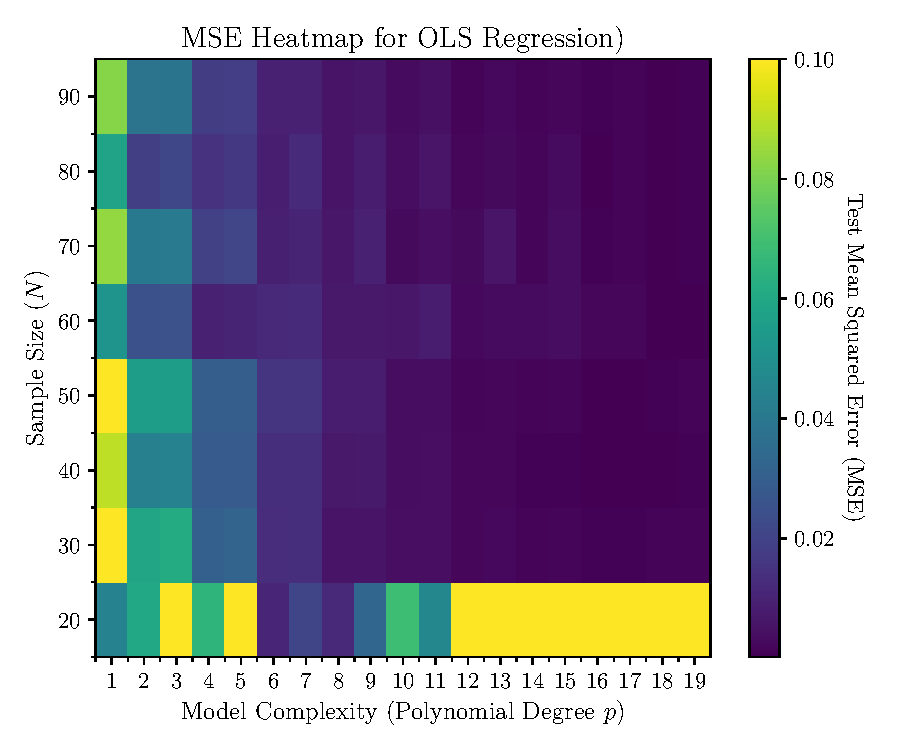
\includegraphics[width=.95 \linewidth]{Figures/OLS_Heatmap.pdf}
    \caption{Training points and Model Complexity}
    \label{fig:OLSHeat}
\end{figure}

\subsubsection{Ridge Regression}
Doing the same training but using Ridge as our method we got some interesting results that elucidates the differences between these models.
Both has there imporvements increasing as the complexity increases the differences are in the lows and the highs.
Where the OLS method\ref{fig:OLS1} had a really low value at degree 10, it also begins to diverge a lot at degree 14.
The Ridge method on the other hand stays remarkably consistent here as seen by the training value. 
Implying that the regularization terms take over and keeps the model from fitting the training data to closely. 

\begin{figure}[h]
    \centering
    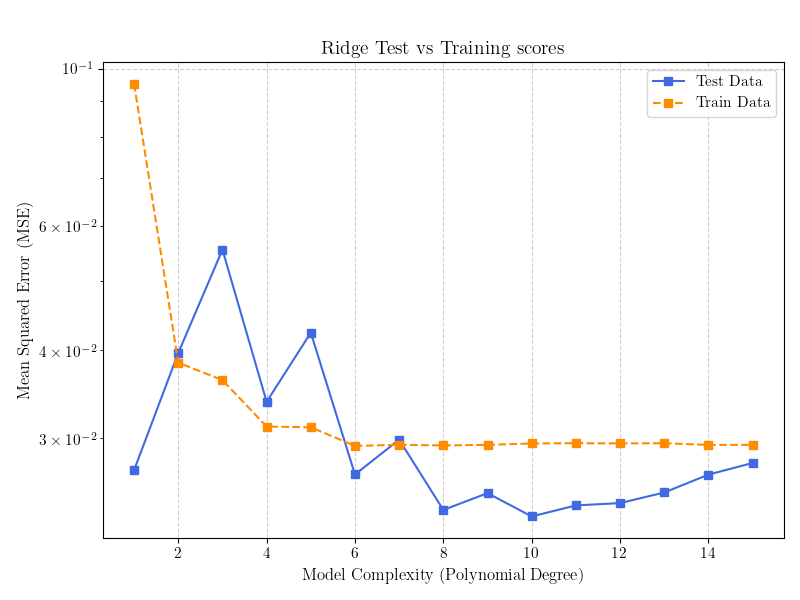
\includegraphics[width=.95 \linewidth]{Figures/MSE_RidgeOnly.png}
    \caption{Ridge and model complexity}
    \label{fig:OLSHeat}
\end{figure}

Now looking closer at the regularization performs with regards to the complexity \ref{fig::} we get that the regularization step cannot be to high as the model will then fail to learn anything and can struggle a bit at lower values when the model complexity increase with the training data.
The model will fit the data to well before the regularization strikes in, though there are some odd lines in this lower right area.


\begin{figure}[h]
    \centering
    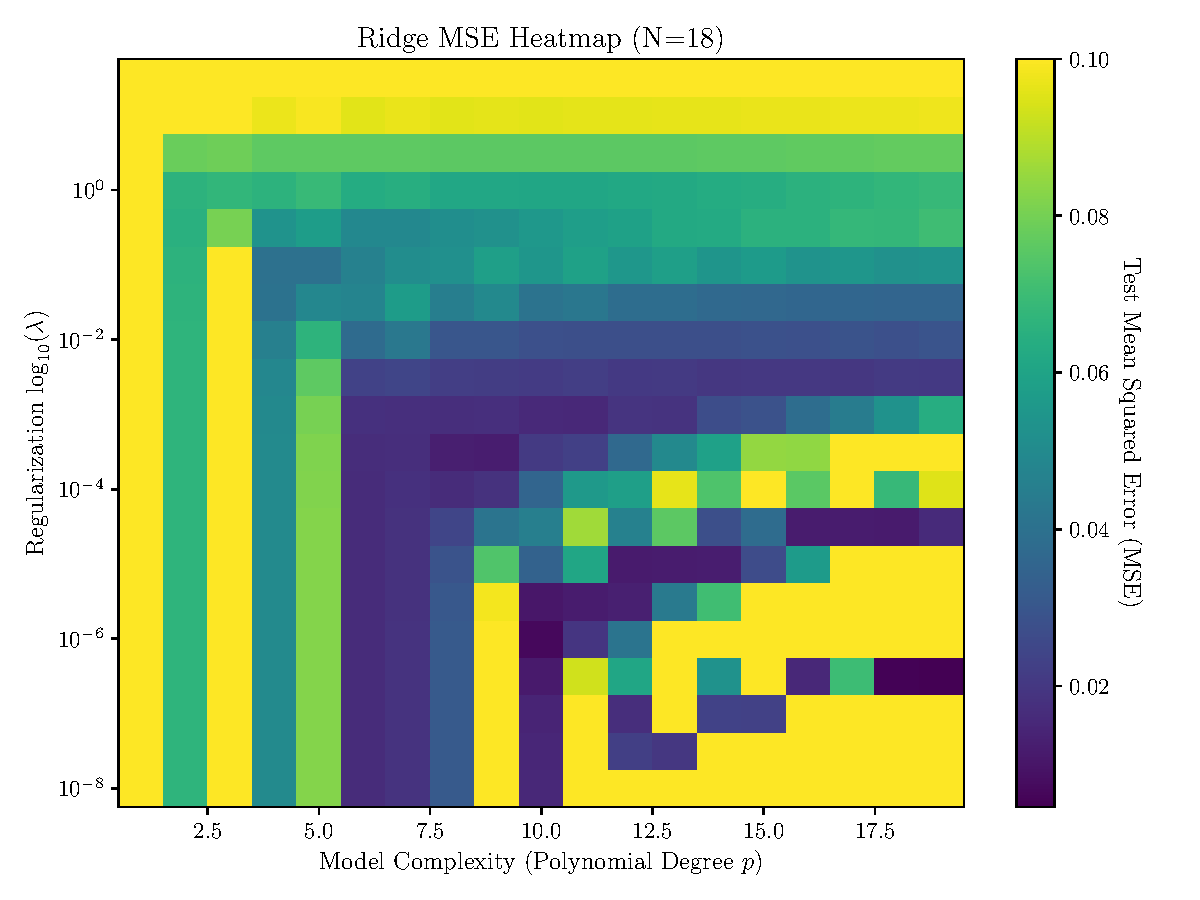
\includegraphics[width=.95 \linewidth]{Figures/Ridge_Degree_Lambda_Heatmap.pdf}
    \caption{Regularization and model complexity}
    \label{fig:}
\end{figure}

\textit{part b}, important to study the dependence on $\lambda$ the regularization parameter

\subsection{Using Gradient Descent}

\subsubsection{OLS and Ridge with gradient descent}
\textit{part c},Study the results from the gradient descent algorithm for both OLS and Ridge regression and especially the dependence on the learning rate $\eta$ and the number of iterations.

\subsubsection{LASSO Regression}
part f, study the results from the stochastic gradient descent algorithm for both OLS and Ridge regression and especially the dependence on the learning rate $\eta$ and the number of iterations.

\subsection{Changing learning rate algorithms}

\subsubsection{Changing learning rate}
\textit{part d}, study the effect of changing the learning rate $\eta$ as a function of the number of iterations. THe methods used for this are momentum, ADAgrad, RMSprop and Adam.
ON all these three regression methods.

\subsubsection{Stochastic Gradient Descent}
Now drag them into the stochastic gradient descent algorithm too see how they develop here.


\subsection{Resampling Techniques}

\subsubsection{Bootstrap}
part g, study the bias-variance tradeoff using the bootstrap method as a resampling technique on the OLS method.

\subsubsection{Cross Validation}
part h, k-fold cross-validation algorithm as a resampling technique on the OLS method. Compare the MSE you get from your cross-validation code with the one you got from your bootstrap code.
Comment and interpret your results.

\begin{comment}
Below you see a picture that describes the Bias-Variance trade off, \ref{fig:BiasVariance1}. 
The trade off here is visualized by having a model of higher complexity molding more and more to the training set thereby having a better fit or bias, but a worse fit on the unseen data.
Which then creates a higher variance.

When you write the results and discussion section you should focus on the following aspects:
\begin{itemize}
    \item Present your results
    \item Give a critical discussion of your work and place it in the correct context.
    \item Relate your work to other calculations/studies
    \item An eventual reader should be able to reproduce your calculations if she/he wants to do so. All input variables should be properly explained.
    \item Make sure that figures\ref{fig:BiasVariance1} and tables contain enough information in their captions, axis labels etc. so that an eventual reader can gain a good impression of your work by studying figures and tables only.
\end{itemize}


\begin{figure}[h]
    \centering
    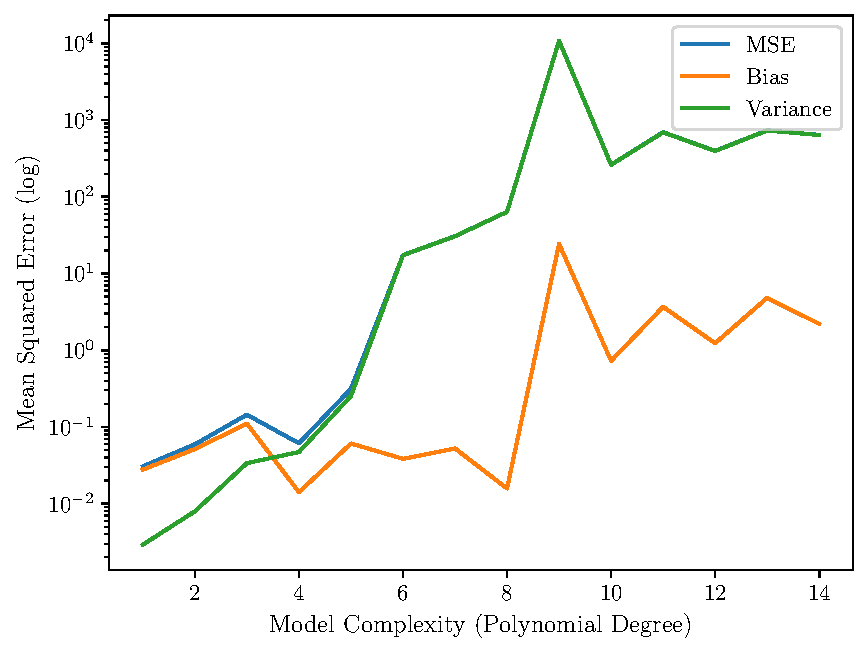
\includegraphics[width=0.9 \linewidth]{Figures/bias_variance_tradeoff.pdf}
    \caption{Bias Variance Tradeoff}
    \label{fig:BiasVariance1}
\end{figure}
Cool reference to the scikit api, \cite{sklearn_api}.


\begin{figure}[h]
    \centering
    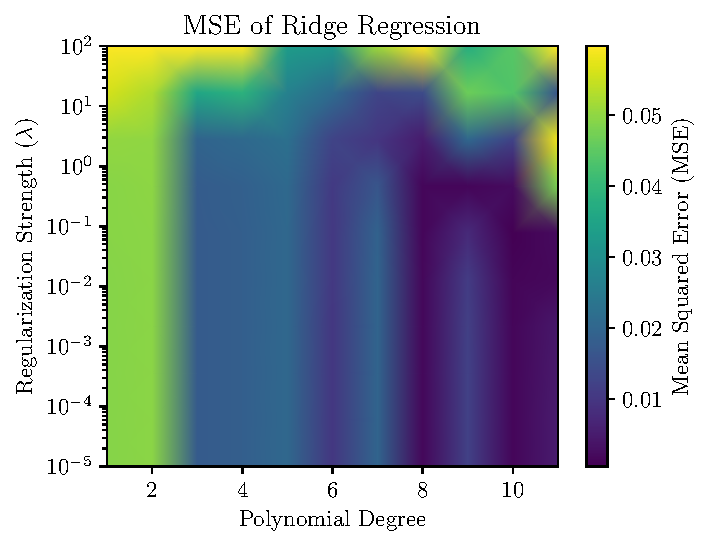
\includegraphics[width=0.9 \linewidth]{Figures/ridge_heatmap.pdf}
    \caption{Degree and Regularization Heatmap}
    \label{fig:DegRegHeat}
\end{figure}
The above heatmap, \ref{fig:DegRegHeat}, implies that a polynomial degree of 8 and a regularization value of slightly above $10^{-1} \lambda$ would be the best parameters for training the model.


\end{comment}

\section{Conclusion}\label{section:conclusion} 
 * State your main findings and interpretations

 * Try as far as possible to present perspectives for future work

 * Try to discuss the pros and cons of the methods and possible improvements
\begin{comment}
When you write the conclusion section you should focus on the following aspects:
\begin{itemize}
    \item State your main findings and interpretations
    \item Try to discuss the pros and cons of the methods and possible improvements
    \item State limitations of the study
    \item Try as far as possible to present perspectives for future work
\end{itemize}

\end{comment}

\bibliography{biblio}



\end{document}
